\subsection{Maquettes}
\paragraph{}
Nous n'allons pas être très original pour se qui est des maquettes, puisqu'il nous est demandé de faire un portage d'Explorer3D vers R, nous allons tout simplement reprendre les mêmes interfaces pour la version.

\paragraph{} Nous allons donc chercher à obtenir d'un coté un panneau latéral de contrôle, grâce à Rgtk, qui contiendra un ensemble de menu, mais aussi de widget tels qu'un slider ou des champs de texte, ou des boutons, des menu déroulants, etc, widgets qui auront pour rôle de lancer les différentes opérations possibles sur les données.\\

\begin{center}
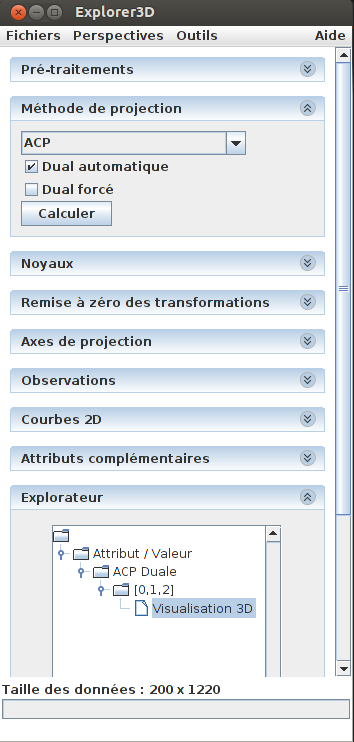
\includegraphics[scale=0.7]{panneau.png}\\
\textit{Aperçu du panneau latéral}\\
\end{center}

\paragraph{} Comme vous pouvez le constater sur l'image précédente, nous somme bien en présence d'un panneau latéral qui offre à l'utilisateur toutes les fonctionnalités du programme sans passer par la console. Nous allons essayer de reproduire au mieux ce panneau, pour offrir aux utilisateurs autant de possibilités que possible.

\paragraph{} Nous allons maintenant parler de la vue 3D, nous l'avons déjà évoqué, elle contient la scène 3D plaqué en 2D à l'écran.\\

\begin{center}
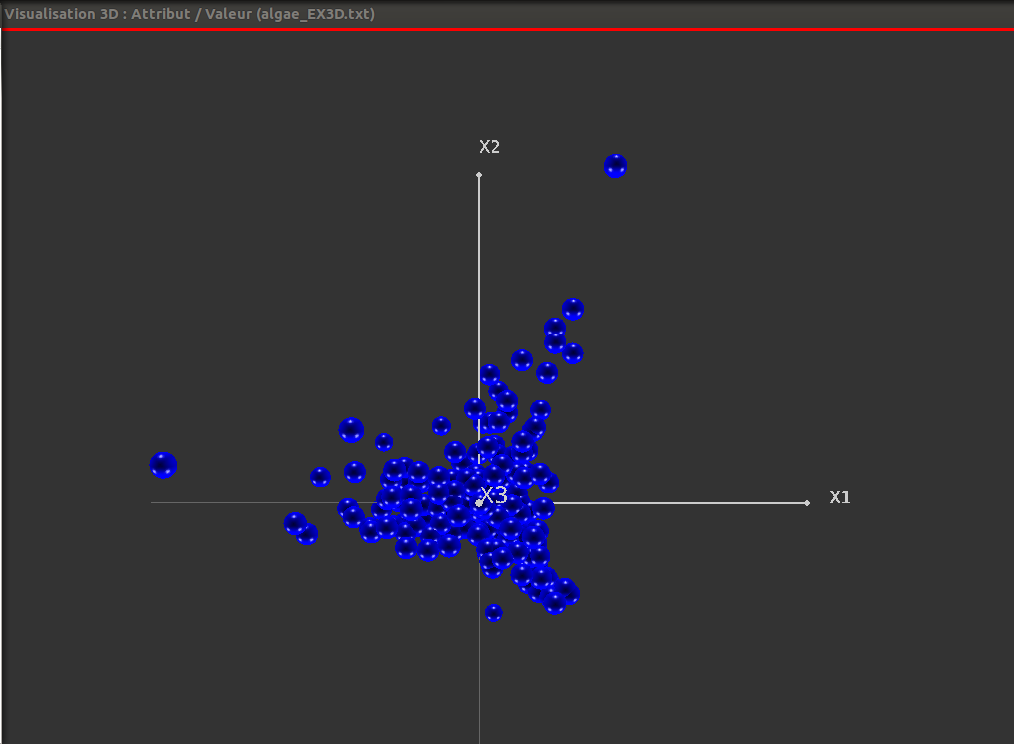
\includegraphics[scale=0.5]{vue3D.png}\\
\textit{Aperçu de la fenêtre 3D}\\
\end{center}

\paragraph{} Cette fenêtre répond déjà à certaines attentes des besoins, à savoir les possibilités de rotation, translation, etc, mais aussi la possibilité de drag/drop, et la possibilité d'afficher un grand nombre d'objet 3D. Il serait souhaitable de pouvoir avoir plusieurs fenêtres simultanément, mais nous n'avons pas encore trouvé ni mis au point un mécanisme permettant de récupérer la fenêtre active. Nous n'allons pas être trop présomptueux sur le sujet, mais cette option si elle s'avère réalisable offrirait à l'utilisateur de plus grandes possibilités, et serait donc plus que bienvenue.
\newpage